\subsection{Deep Learning}
Deep learning is a branch of machine learning. The main difference between the use of machine learning and deep learning, is that deep learning is more suitable for handling raw data forms. Instead, a machine learning system often needs a feature extractor, that will generate a feature vector from the data that can be used as an input.
Deep learning is based on different techniques that makes it able to handle raw data, mainly because of its structure.\citep{LeCun2015, Schmidhuber2015} Because of this the system will automatically detect the necessary representations needed for classification and detection. \newline
Neural network is a structure of deep learning which consists of different layers, that can be divided into input- and output-layers, with one or more hidden layers in between \citep{Schmidhuber2015}. The key aspect of these layers is that the features are not defined by programmers, but they are found and learned from raw data using a general–purpose learning procedure.\citep{LeCun2015} An example of a neural network structure can be seen in figure \ref{fig:NN_structure}.   

\begin{figure} [H]
\centering
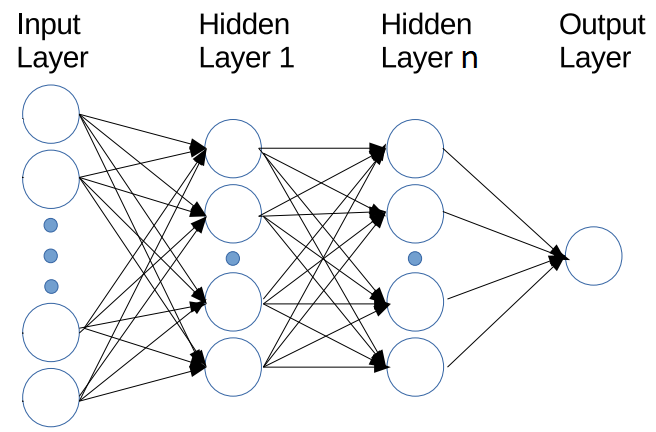
\includegraphics[width=0.6\textwidth]{figures/NN_structure}
\caption{Example of the structure of a neural network. Edited \citep{Acquarelli2017}.}
\label{fig:NN_structure}  
\end{figure}

\noindent
The different layers consist of a series of nodes, where each node is connected by weights ****EXPLAIN!!*** to one or several other nodes in different layers. In the input-layer the nodes receive data. The second layer will then receive the output from the previous layer, and this process continues through the layers until the output-layer is reached.\citep{Schmidhuber2015} An example of how the hidden layers may affect an image in one type of neural network can be explained in the following.  
Firstly, the system detects minor changes like edges. Secondly, the edges are compared and put together to make up different kind of shapes. In the third hidden layer, it will be further combined to make up an object that can be identified.\citep{LeCun2015}

%Maybe explain a bit more to how the different nodes contain activation functions...

% Maybe explain how the input becomes the output in a litte more detail.  The weights are interconnection between two layers and they work as a set of coefficients, defining an image feature.\citep{Hameed2016}

% The following is already discriped in back prop, but could be used earlier or later maybe - By adjusting weights in the neural network it is possible to fit the model better to the training data, and thereby increase its accuracy and reduce error \citep{LeCun2015}.

\subsubsection{Learning scenarios}
****WRITE A INTRODUCTION! ITS NEED TO BE TRAIN, OPTIMIZED ECT.*****
There are different approaches for training a neural network, where the two main learning scenarios are supervised and unsupervised learning.

\noindent
Supervised learning is the most common way of training in machine learning. When applying this learning method the neural network is trained with input data that has a corresponding label. The network calculates an output through the forward pass, where the data is simply passed through the network. This output may then be compared to the label, and used to evaluate the performance of the system. As a result of the evaluation, the network may learn form the data by doing a backward pass through the network, also known as back-propagation.\citep{LeCun2015} Overall supervised learning may be described as teaching the network how to associate a given input to a specific output \citep{Goodfellow2016}, and is mostly associated with classification, regression, and ranking problems \citep{Mehryar2012}. 

\noindent
Unsupervised learning is when training is performed with data that has no output label. Instead of learning associations between input and output, the network organizes the data by searching for common characteristics \citep{Mehryar2012}. An example of an unsupervised learning algorithm is k-mean clustering, where the unlabeled dataset goes through a classification, and splits data into clusters that are near each other \citep{Goodfellow2016}.  

%\noindent
%\textbf{Semi-supervised learning} network receives both labeled, unlabeled data and then it searches for common characteristics in data. It is used mainly when the labeled data is hardly collected and unlabeled data is easily reachable. \citep{Mehryar2012}

  
\subsection{Back-propagation}
***** CORRECT FORWARD AND BACKWARD + EQUATIONS******
Back-propagation is a popular learning algorithm in neural networks, that is based on gradient descent, and used because of it's simplicity and computationally efficiency.\citep{Bengio2012, Duda2000} It is the learning process where the weights of a neural network are adjusted in order to reduce the error calculated between the calculated output of the network and the expected output. This makes back-propagation closely related to supervised learning, to which back-propagation is the most general method used.\citep{Duda2000}  
When a neural network is initialized the weight may be set with a random value, meaning that the neural network may perform very poorly through the first iterations of the training. Based on a loss function a loss is calculated for every input that passes through the network, that may be used as a part of back-propagation to make the adjustments on the weights to reduce this loss. As training progresses, the loss should decrease as a result of the weight adjustments, and improve the performance of the neural network.\citep{LeCun2015, Goodfellow2016, Duda2000}   
This learning process continues until optimal weights with minimum error is reached.\citep{Hameed2016}
\noindent
The basic concept is that gradients can be computed efficiently by propagation from the output to the input in order to minimize the overall output error as much as possible during the learning stage. This algorithm process is divided in two main stages: forward and backward. In the first process (forward), the back-propagation architecture is described as the inputs and weights multiplication of separate node summed with additional coefficient called bias.\citep{Hameed2016,LeCun1998} \\

MAYBE TALK ABOUT ACTIVATION FUNCTIONS IN RELATION TO BACKPROPAGATION. 

IF WE WILL HAVE TIME WE NEED TO ADD ACTIVATION GRAPHS WITH EXPLANATION

A PROBLEM OFTEN RELATED TO OPTIMIZATION IS THE LAGER THE NETWORK THE HARDER IT IS TO OPTIMIZE, BUT IN ANOTHER WAY IF THE NETWORK IS SMALL AND SIMPLE THE EASIER IT IS TO OPTIMIZE. 


\subsubsection{Gradient Descent}
Gradient descent is one of the most common techniques for optimizing neural networks. It is a way to minimize the loss function by updating the parameters, like weights, in the opposite direction of the gradient of the objective function.\citep{Ruder2016} The principle of the gradient descent could be explained as a "ball climbing down a hill" until a local minimum is reached as shown in figure \ref{fig:GDgraph}. At each step, the opposite direction of the gradient is taken and the step size is determined by the value of the learning rate together with the slope of the gradient until the convergence is reached. Convergence means that oscillations of the value are small enough to call it the minimum value.\citep{Raschka2016}

\begin{figure} [H]
\centering
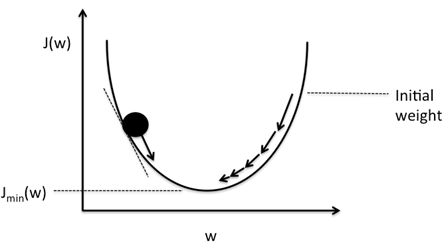
\includegraphics[width=0.6\textwidth]{figures/GDgraph}
\caption{Illustration of gradient descent working principle, where J(w) is the loss function, Jmin(w) is final approximation to the local minimum of J(w), w is value of the parameter. The arrows indicate the step direction, i.e. the negative gradient.\citep{Raschka2016}}
\label{fig:GDgraph}  
\end{figure}

\noindent
There are three variants of gradient descent: batch gradient descent, stochastic gradient descent, and mini-batch gradient descent. They differ on the amount of data used to compute the gradient of the loss function. Depending on which of the gradient descent variants is used, the trade-off between the accuracy and the runtime could be seen.

\noindent
Batch gradient descent computes the gradient of the cost function with regards to the parameters for the entire training dataset.\citep{Ruder2016} Batch gradient descent has the significant deficiency, it takes a single step for one pass over the training set, meaning the larger dataset, the slower algorithm updates the weights and the longer it will take to reach global minimum.[quota] In cases like these, stochastic gradient descent is being used more commonly. **** SOURCE ****

\noindent
Stochastic gradient descent (SGD) performs a parameter update for each training example and label. It is therefore much faster and it also performs frequent updates with a high variance causing loss function to fluctuate. These fluctuations enable it to jump to new potentially better local minima, but it may complicate the convergence to reach the exact minimum because of overshooting.\citep{Zhang2014}

\noindent
Mini-batch gradient descent performs the parameters update for every mini-batch of training examples, specified by a batch size. By that, the variance of the parameter updates are reduced leading to more stable convergence and fast performance.\citep{Ruder2016}

\noindent
Additionally, there could be few challenges while using gradient descent as an optimizer. It is difficult to pick a proper learning rate so few gradient descent optimization algorithms were invented. The most popular optimizers are adagrad, adadelta and adam. **** SOURCE ****

%\noindent
%Momentum is a method for accelerating SGD in a relevant direction and for reduction of oscillations. As a result, faster convergence is obtained but there is a risk of overshooting the minimum value.\citep{Qian1999}

\noindent
Adagrad is an algorithm for gradient descent optimization which adapts the learning rate to the parameters. It performs larger updates for frequent and smaller for infrequent features. It has one weakness if the learning rate shrinks too much, the algorithm is no longer able to adapt.\citep{Ruder2016}

\noindent
Adadelta is an updated version of Adagrad, but the learning rate is monotonically decreasing. Using this optimizer, there is no need to tune the parameters of optimizer meaning that it can be applied in a variety of situations.\citep{Ruder2016}

\noindent
Adam stands for Adaptive Moment Estimation. It is the most used method for computing adaptive learning rate and updating the parameters.  This optimizer calculates the learning rate for each parameter and stores momentum changes separately. This helps to reach the convergence faster with a decent learning speed.\citep{Kingma2015}\\

\noindent
A study \citeauthor{Patacchiola2017} showed the evaluation of the performance on different optimizers on a dataset containing 21977 female and male head pose images. The result is shown in figure \ref{fig:Graphofyrainingcost}, where the Adam optimizer had the fastest convergence rate and it reached the lowest loss values. 

\begin{figure} [H]
\centering
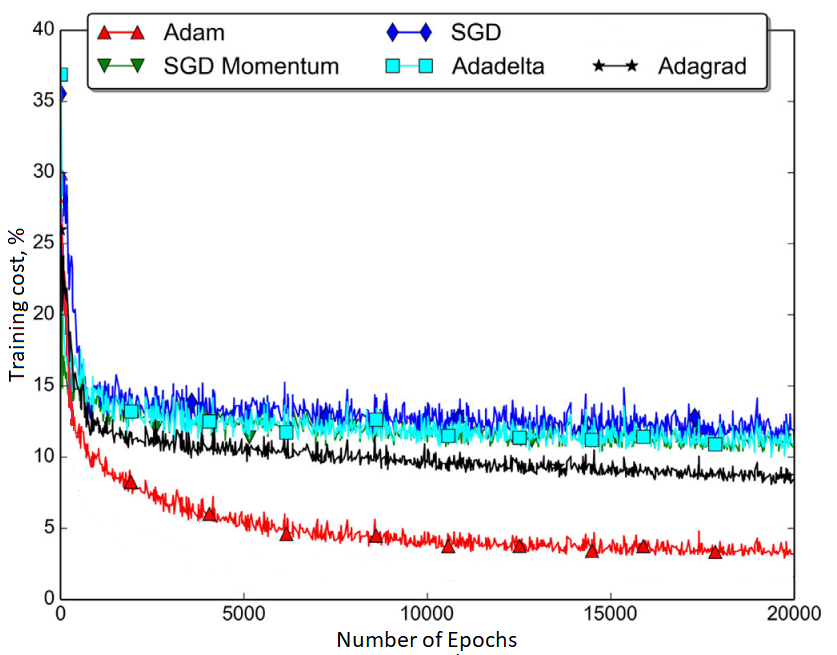
\includegraphics[width=0.6\textwidth]{figures/Graphofyrainingcost}
\caption{Comparison of the convergence speed between different optimizers used to train architecture on ALFW dataset. The loss values are the mean of the five attempts.\citep{Patacchiola2017}}
\label{fig:Graphofyrainingcost}  
\end{figure}

\noindent
However, the results are not always similar. All of the optimizers perform differently depending on the problem and parametrization, which in the majority of the cases is the most challenging part. This leads to the conclusion that there are not a winning optimizer and it has to be chosen based on every problem.\citep{Int82016}

% Mention local minima and gobal minima and why it is not so importent to find the absolute global minima \citep{Duda2000}. 

% Mention the mini bacthes are used in order to reduce the computation cost, and that the size of the mini-batch is often what limits the network computation. , mini-batches and optimizers



\subsubsection{Learning curves}
**** EXPLAIN WHY IT'S GOOD TO SEPARATE DATA AND WHY? MOVE IT UP BEFORE GRADIENT  ****
During the beginning of training, the training error of network will typically be relatively high, but during training the error decreases monotonically, as the weights are adjusted in the network \citep{Duda2000}. An illustration of how the error values are affected during training can be seen in figure \ref{fig:learningCurve}.

\begin{figure} [H]
\centering
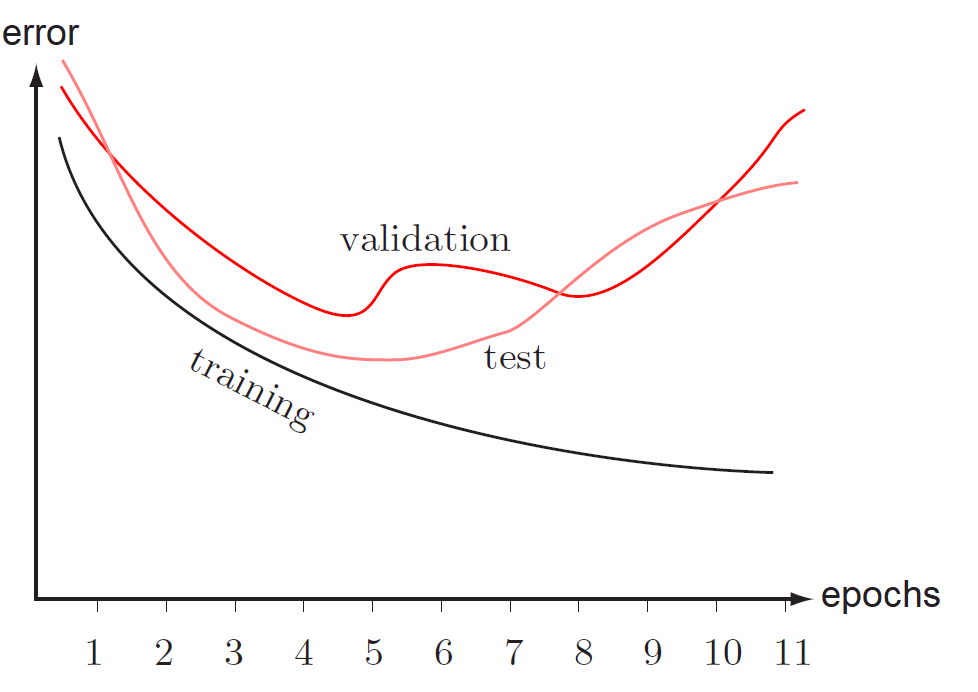
\includegraphics[width=0.7\textwidth]{figures/learningCurves}
\caption{Illustration of how training (black), validation (red), and test (orange) error is affected by the increase in epochs. Edited \citep{Duda2000}.}
\label{fig:learningCurve}
\end{figure}

\noindent
From the figure it can be seen how the error value of the validation, can be used to evaluate the network. 
Near the fifth epoch the validation and the test error starts to rise, indicating that the network is overfitting to the training data, thereby decreasing the generalization abilities. 
Validation error can therefore be used as stop criterion for when the training is optimal, and prevent overfitting. 
Typically the validation and test error will always be higher than the training error, which is also seen in figure \ref{fig:learningCurve}.\citep{Duda2000}

\subsection{Dropout}\label{sec:dropout}
Dropout is a regulation technique used to reduce overfitting of the neural network. In a network the dropout is applied to the individual layers, and works by randomly dropping different nodes temporarily in the given layer during training. An illustration of the principle of dropout can be seen in figure \ref{fig:Dropout}. This parameter is specified with a percent value, which defines the fraction of the nodes that drop \citep{Chollet2015}.

\begin{figure} [H]
\centering
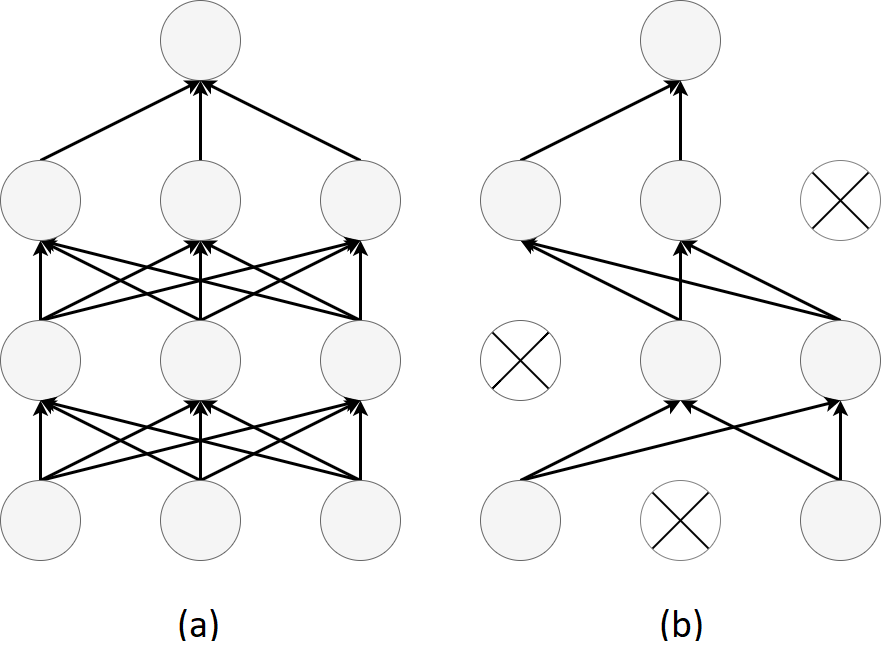
\includegraphics[width=0.6\textwidth]{figures/Dropout}
\caption{Dropout effect: The figure on the left illustrates a fully connected network, without dropout, and the right shows a network where dropout is enabled on the first three layers. Edited \citep{Srivastava2014}.}
\label{fig:Dropout} 
\end{figure}

\noindent
This reduces co-adaptation, where nodes compute the same features, to where this may increase the generalization capabilities for a neural network. 
A study \citeauthor{Srivastava2014} has tested the use of dropout in different neural networks, and indicates that the most optimal range of dropout is 20\% of the nodes in the visible layers, and 50\% in the hidden layers.\citep{Srivastava2014}

\subsection{Core Neural Network layers}
**** INTRODUCTION! ****

\subsubsection{Convolutional Neural Networks}
Convolutional Neural Networks (CNNs) is a type of special neural network for processing data with a grid-like topology \citep{Goodfellow2016}. CNNs perform highly in several tasks, including digit recognition, image classification and face recognition. The key aspect of CNNs is to automatically learn a complex pattern by extracting visual features from the pixel-level content.\citep{Acquarelli2017,LeCun1998}

\noindent
The architecture of a typical CNNs is always combined of two types of layers: convolutional and pooling \citep{Goodfellow2016, LeCun2015}. 

\noindent
The purpose of the convolutional layer is to recognize the features in the input by taking e.g. an image and scan it, then split it up into the feature maps. The terminology regarding the output of a convolutional layer can be referred to a feature map \citep{Goodfellow2016,LeCun1998}. A complete convolutional layer consists of several feature maps, so multiple features can be extracted at each location in the image \citep{LeCun1998}. 
%It usually consists of few features maps, where each map represents different feature. 
The other layer called pooling, typically follows after convolutional layer. It consists of the same number of feature maps as the previous convolutional layer had. Each feature map is used as a new input in a pooling layer. Depending on the network's depth, the convolutional and pooling layers alternate until the last pooling layer is reached.\citep{LeCun1998}

\noindent
The combination of convolutional and pooling layers defines the part of the network which performs feature extraction while the classification part is made by fully connected layers. 
\noindent
A typical CNNs architecture for character recognition of the images, called LeNet-5, can be seen in figure \ref{fig:LeNet5}.


%
%Units in a layer are organised in planes and share the same set of weights \citep{LeCun1998}.
%CNNs are feed–forward models that map input data with a set of suitable outputs. Accuracy and performance rely on large training datasets and training procedure based on back-propagation with optimization algorithm such as gradient descent which is used for finding minimum value of the function.\citep{Acquarelli2017}
 
\begin{figure} [H]
\centering
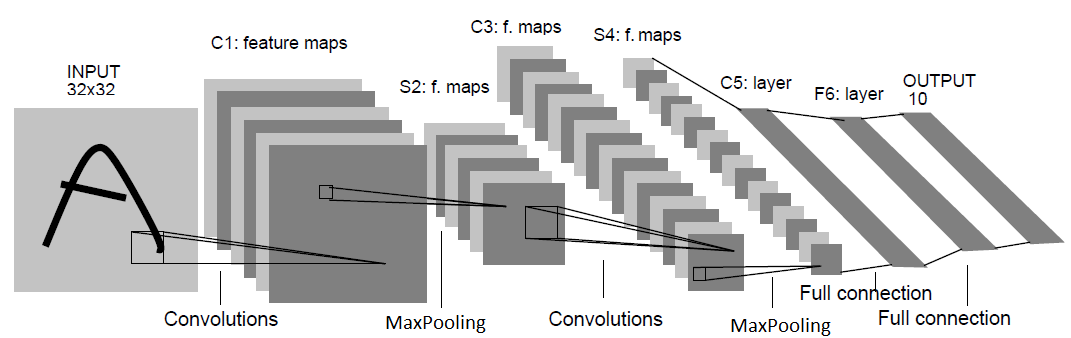
\includegraphics[width=1.0\textwidth]{figures/LeNet5}
\caption{Architecture of LeNet-5, a CNN for character recognition. Each plane is a feature map and the size of the feature map differs throughout the layers. The model consists of two convolutional, two pooling and two fully connected layers \citep{LeCun1998}.}
\label{fig:LeNet5}  
\end{figure}
% The feature map is made by scanning the input image with a single unit that has a local respective field and store the state of this unit in the new feature map (new layer) and this process is called convolution.Respective field term is defined as the region in the input space that a particular CNN's feature is looking at.

\noindent
Units in the first hidden layer of LeNet-5 are arranged in planes, which are a separate feature maps respectively. Once a feature has been detected, its location becomes unimportant and only its approximate position relative to other features is relevant. This is because the positions are likely to vary for different images of the same object and it is irrelevant for identifying the pattern. To reduce the importance of the position, the spacial resolution of the feature map is decreased by the use of pooling layer.\citep{LeCun1998}


%Additional explanation of the example in start of deep learning (How it first detects edges and then shape and then objects. )

\subsubsection{Pooling layer} ***MOVING THE EXAMPLE TO THE END, SO CNN IS FIRST, THEN POOLING, FULLY CONNECTED LAYERS AND THE EXAMPLE***
As previously mentioned convolution are typically followed by pooling \citep{LeCun2015, Goodfellow2016}. 
Pooling can be used to reduce the size of the dataset, which may increase computation speed, because the amount of data passed to the next layer is smaller. By pooling the input, a smaller representation is given, that still contains the relevant features.\citep{Goodfellow2016,LeCun1998}   
\noindent  
The pooling process can be defined as a window that passes over e.g. a feature map from convolution, where a value within the window is extracted. One type of pooling layer is max pooling that takes the maximum value within the window \citep{Goodfellow2016, Dumoulin2016}. A pooling layer may be defined simply by its window (Kernel) size, paddling size and a stride length, where stride length is the number of values the window jumps as shown in figure \ref{fig:Kernel}.\citep{Dumoulin2016}


\begin{figure} [H]
\centering
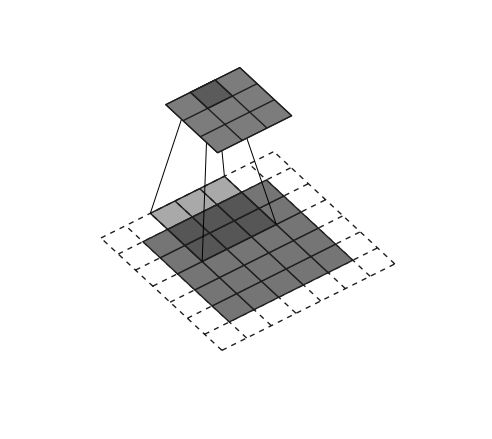
\includegraphics[width=0.25\textwidth]{figures/Kernel}
\caption{Illustration of pooling with 3x3 kernel over a 5x5 input using paddling and strides (i.e., input = 5, kernel = 3, stide = 1, paddling size = 1) \citep{Dumoulin2016}.}
\label{fig:Kernel}  
\end{figure}